\documentclass[11pt,a4paper]{article}

\usepackage[indonesian]{babel}
\usepackage{fontspec}
\setmainfont{Times New Roman}
\setsansfont{Arial}
\setmonofont{Consolas}[Scale=0.88]

\usepackage[top=2.5cm,bottom=2.3cm,left=2.6cm,right=2.4cm,headheight=14pt]{geometry}
\usepackage{graphicx}
\usepackage{xcolor}
\usepackage{titlesec}
\usepackage{fancyhdr}
\usepackage{lastpage}
\usepackage{tabularx}
\usepackage{array}
\usepackage{colortbl}
\usepackage{enumitem}
\usepackage{setspace}
\usepackage{parskip}
\usepackage{needspace}
\usepackage{tikz}
\usetikzlibrary{arrows.meta,positioning,shapes.geometric}
\usepackage{listings}
\usepackage{hyperref}

\definecolor{PolibatamBlue}{HTML}{2F5496}
\definecolor{TableHeadBg}{HTML}{E8EEF6}
\definecolor{RowShade}{HTML}{F5F7FA}
\definecolor{JajanGreen}{HTML}{2E8B3D}
\definecolor{ActorFill}{HTML}{F0F6FC}

\lstset{
  basicstyle=\ttfamily\fontsize{8.5}{10.5}\selectfont,
  backgroundcolor=\color{RowShade},
  frame=single,
  rulecolor=\color{PolibatamBlue},
  breaklines=true,
  columns=fullflexible,
  keepspaces=true,
  showstringspaces=false,
  commentstyle=\color{JajanGreen}\itshape,
  keywordstyle=\color{PolibatamBlue}\bfseries,
  stringstyle=\color{black!75}
}

\hypersetup{
  colorlinks=true,
  linkcolor=PolibatamBlue,
  urlcolor=PolibatamBlue,
  pdftitle={Dokumentasi Implementasi Fitur F006 dan F007 - JajanRia}
}

\titleformat{\section}
  {\normalfont\fontsize{13}{16}\bfseries}
  {\textcolor{PolibatamBlue}{\thesection.}}
  {0.6em}
  {}
\titleformat{\subsection}
  {\normalfont\fontsize{11.5}{14}\bfseries}
  {\textcolor{PolibatamBlue}{\thesubsection}}
  {0.6em}
  {}

\titlespacing*{\section}{0pt}{12pt}{5pt}
\titlespacing*{\subsection}{0pt}{8pt}{3pt}

\newcolumntype{L}[1]{>{\raggedright\arraybackslash}p{#1}}
\newcolumntype{C}[1]{>{\centering\arraybackslash}p{#1}}
\newcolumntype{Y}{>{\raggedright\arraybackslash}X}

\fancypagestyle{plain}{%
  \fancyhf{}%
  \renewcommand{\headrulewidth}{0pt}%
  \renewcommand{\footrulewidth}{0pt}%
  \fancyfoot[C]{%
    \fontsize{9}{11}\selectfont\sffamily
    \begin{tabular*}{\textwidth}{@{}l@{\extracolsep{\fill}}c@{\extracolsep{\fill}}r@{}}
      Dokumentasi Teknis JajanRia (PBL-TRPL104) & Fitur F006 \& F007 & Halaman \thepage{} dari \pageref{LastPage}
    \end{tabular*}%
  }%
}
\pagestyle{plain}

\begin{document}
\setstretch{1.15}
\emergencystretch=2em

% === HEADER DOKUMEN ===
\noindent
\begin{tabularx}{\textwidth}{@{}C{2.0cm}Y@{}}
  \raisebox{-0.45\height}{
\includegraphics[width=1.7cm]{assets/polibatam_logo.png}} &
  {\sffamily\bfseries\fontsize{15}{18}\selectfont\color{PolibatamBlue} Dokumentasi Workflow \& Implementasi Fitur F006 dan F007}\\[3pt]
  & {\sffamily\small Platform E-Commerce Kuliner Kampus \textbf{JajanRia} (Semi-Automated Direct Commerce)}\\
  & {\sffamily\footnotesize Ruang Lingkup: Keranjang per Lapak, \textit{Checkout}, Unggah Bukti Bayar, \& Validasi Server \textbullet{} 23 November 2026}
\end{tabularx}
\vspace{0.15cm}
{\color{JajanGreen}\hrule height 1.5pt}
\vspace{0.35cm}

\section{Ringkasan Spesifikasi Fitur F006 dan F007}

Fitur \textbf{F006} dan \textbf{F007} merupakan inti transaksi langsung (\textit{Direct Commerce}) pada skenario \textit{Use Case} \textbf{UC-03}, yang menggantikan pemesanan manual via obrolan dengan pencatatan pesanan terstruktur ke tabel \texttt{t\_pesanan} serta verifikasi pembayaran manual tanpa gerbang pembayaran pihak ketiga.

\renewcommand{\arraystretch}{1.22}
\begin{tabularx}{\textwidth}{|C{1.1cm}|L{2.9cm}|Y|L{4.4cm}|}
\hline
\rowcolor{TableHeadBg}
\textbf{Kode} & \textbf{Nama Fitur} & \textbf{Aturan Bisnis \& Validasi Utama} & \textbf{Berkas Terkait} \\
\hline
\textbf{F006} & Keranjang per Lapak \& \textit{Checkout} Mandiri & Keranjang terpisah per \texttt{id\_umkm}; subtotal dan \texttt{total\_harga} dihitung ulang di server dari \texttt{t\_produk}; \texttt{catatan\_pembeli} disimpan; menu habis (\texttt{tersedia=false}) ditolak \texttt{HTTP 422}. & \texttt{store-detail.blade.php}, \texttt{ChatController.php} (\texttt{checkoutOrder}) \\
\hline
\textbf{F007} & Unggah Foto Bukti Pembayaran & Unggah foto transfer/QRIS (\texttt{jpg/jpeg/png}, maks.\ 3 MB) opsional saat \textit{checkout} atau susulan/ulang via laci \textit{History Pesanan}; unggah ulang ditolak \texttt{HTTP 400} jika status sudah \textit{lunas}. & \texttt{floating-chat.blade.php}, \texttt{ChatController.php} (\texttt{uploadBuktiPembayaran}) \\
\hline
\end{tabularx}

\section{Workflow End-to-End F006 dan F007}

Gambar~\ref{fig:wf-f006-f007} memvisualisasikan alur kerja lengkap mulai dari pemilihan menu di halaman detail lapak hingga penyimpanan pesanan dan unggah bukti pembayaran.

\begin{figure}[htbp]
\centering
\resizebox{\textwidth}{!}{%
\begin{tikzpicture}[
  box/.style={draw=PolibatamBlue, thick, rounded corners=3pt, fill=ActorFill, minimum width=3.1cm, minimum height=1.0cm, align=center, font=\sffamily\scriptsize, inner sep=4pt},
  srv/.style={draw=JajanGreen, thick, rounded corners=3pt, fill=green!6, minimum width=3.2cm, minimum height=1.0cm, align=center, font=\sffamily\scriptsize, inner sep=4pt},
  err/.style={draw=red!70!black, thick, rounded corners=3pt, fill=red!6, minimum width=2.7cm, minimum height=0.9cm, align=center, font=\sffamily\scriptsize, inner sep=4pt},
  arr/.style={->, >=Stealth, thick, PolibatamBlue},
  earr/.style={->, >=Stealth, thick, red!70!black},
  lbl/.style={font=\sffamily\tiny\bfseries, fill=white, inner sep=1pt}
]
  % Baris 1: Frontend F006
  \node[box] (cart) at (0, 0) {\textbf{1. Detail Lapak (UI)}\\Tambah/kurang porsi\\(\texttt{localStorage} per UMKM)};
  \node[box] (modal) at (4.4, 0) {\textbf{2. Modal Checkout}\\Isi \texttt{catatan} \& pilih\\foto bukti (opsional)};
  \node[srv] (val) at (9.0, 0) {\textbf{3. Validasi Server}\\Cek sesi, lapak aktif,\\\& \texttt{tersedia=true}};
  \node[err] (rej1) at (13.3, 0) {\textbf{Tolak Menu Habis}\\(\texttt{HTTP 422} / \texttt{401})};

  % Baris 2: Simpan Pesanan & Cabang F007
  \node[srv] (calc) at (9.0, -2.3) {\textbf{4. Hitung \& Simpan}\\Hitung \texttt{total\_harga} dari DB,\\simpan ke \texttt{t\_pesanan}};
  \node[box] (hasfoto) at (4.4, -2.3) {\textbf{5a. Ada Bukti Foto?}\\Ya: \texttt{menunggu\_verifikasi}\\Tidak: \texttt{belum\_bayar}};
  \node[box] (hist) at (0, -2.3) {\textbf{6. Laci History Pesanan}\\Pantau status \& klik\\``Upload/Perbarui Bukti''};

  % Baris 3: Upload Bukti Susulan (F007)
  \node[srv] (up) at (4.4, -4.9) {\textbf{7. Upload Bukti Bayar}\\Cek kepemilikan \&\\status $\neq$ \texttt{lunas}};
  \node[err] (rej2) at (0, -4.9) {\textbf{Tolak Jika Lunas}\\(\texttt{HTTP 400})};
  \node[srv] (done) at (9.0, -4.9) {\textbf{8. Siap Diverifikasi}\\Simpan ke \texttt{storage/public},\\status: \texttt{menunggu\_verifikasi}};

  % Panah Baris 1
  \draw[arr] (cart) -- node[lbl, above] {Checkout} (modal);
  \draw[arr] (modal) -- node[lbl, above] {\texttt{FormData}} (val);
  \draw[earr] (val) -- node[lbl, above] {Gagal} (rej1);

  % Panah Baris 1 -> 2
  \draw[arr] (val.south) -- node[lbl, right] {Lolos} (calc.north);
  \draw[arr] (calc.west) -- (hasfoto.east);
  \draw[arr] (hasfoto.west) -- node[lbl, above] {Tampil} (hist.east);

  % Panah Baris 2 -> 3 (jalur bersih melalui atas blok 7 agar tidak menimpa panah Tolak)
  \draw[arr] (hist.south) -- (0, -3.6) -| node[lbl, above, pos=0.25] {Unggah susulan} (up.north);
  \draw[earr] (up.west) -- node[lbl, above] {Lunas} (rej2.east);
  \draw[arr] (up.east) -- node[lbl, above] {Valid} (done.west);
\end{tikzpicture}%
}
\caption{Diagram \textit{Workflow} Fitur F006 (\textit{Checkout}) dan F007 (Unggah Bukti Pembayaran)}
\label{fig:wf-f006-f007}
\end{figure}

\section{Tahapan Implementasi Frontend}

\subsection{Keranjang per Lapak dan Modal Checkout (\texttt{store-detail.blade.php})}
Implementasi sisi klien pada halaman detail toko memisahkan keranjang tiap UMKM agar pesanan dari dua lapak berbeda tidak tercampur:
\begin{enumerate}[leftmargin=1.5em, itemsep=2pt, topsep=2pt]
  \item \textbf{Penyimpanan Keranjang Lokal:} kunci \texttt{localStorage} dibentuk unik per \texttt{umkmId} (\texttt{cartKey}), menyimpan objek \texttt{items[id\_produk]} berisi \texttt{id\_produk}, \texttt{nama\_produk}, \texttt{harga}, dan \texttt{qty}.
  \item \textbf{Kontrol Porsi (\texttt{tambahKeKeranjang}, \texttt{ubahQtyItem}, \texttt{updateCartUI}):} menekan tombol tambah atau tombol \texttt{+} / \texttt{-} memperbarui \texttt{qty}, menghapus entri jika \texttt{qty <= 0}, serta menyinkronkan bilah keranjang mengambang (\texttt{\#floatingStoreCart}). Menu yang berstatus habis tidak memiliki tombol tambah aktif.
  \item \textbf{Modal \textit{Checkout} (\texttt{bukaModalCheckout}, \texttt{previewBuktiCheckout}):} memeriksa status sesi masuk; jika valid, merender ringkasan item memakai node DOM aman (\texttt{textContent}), mereset \texttt{\#checkoutCatatan}, serta memvalidasi berkas foto bukti transfer maksimal 3~MB sebelum menampilkan pratinjau \texttt{FileReader}.
  \item \textbf{Pengiriman Asinkron (\texttt{kirimDedicatedCheckout}):} membungkus \texttt{id\_umkm}, \texttt{items} (JSON string), \texttt{catatan}, dan \texttt{bukti\_foto} ke dalam \texttt{FormData}, lalu mengirim permintaan \texttt{POST} ke rute \texttt{api.orders.\allowbreak checkout} dengan token CSRF. Jika sukses, keranjang lokal dibersihkan dan modal sukses ditampilkan.
\end{enumerate}

\begin{figure}[htbp]
\centering
\begin{minipage}[t]{0.48\textwidth}
  \centering
  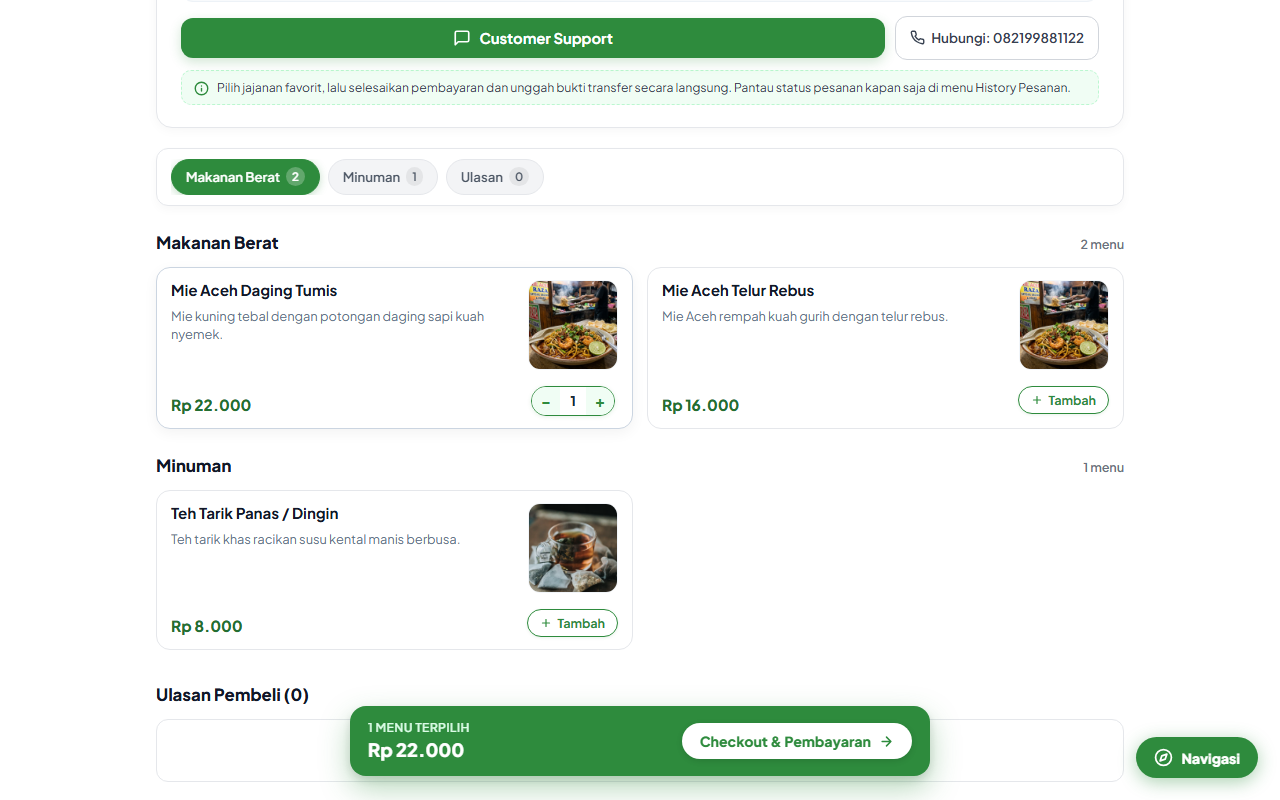
\includegraphics[width=\textwidth]{assets/screens/04_store_detail.png}
  \par\small (a) Detail Lapak \& Keranjang Mengambang (F006)
\end{minipage}\hfill
\begin{minipage}[t]{0.48\textwidth}
  \centering
  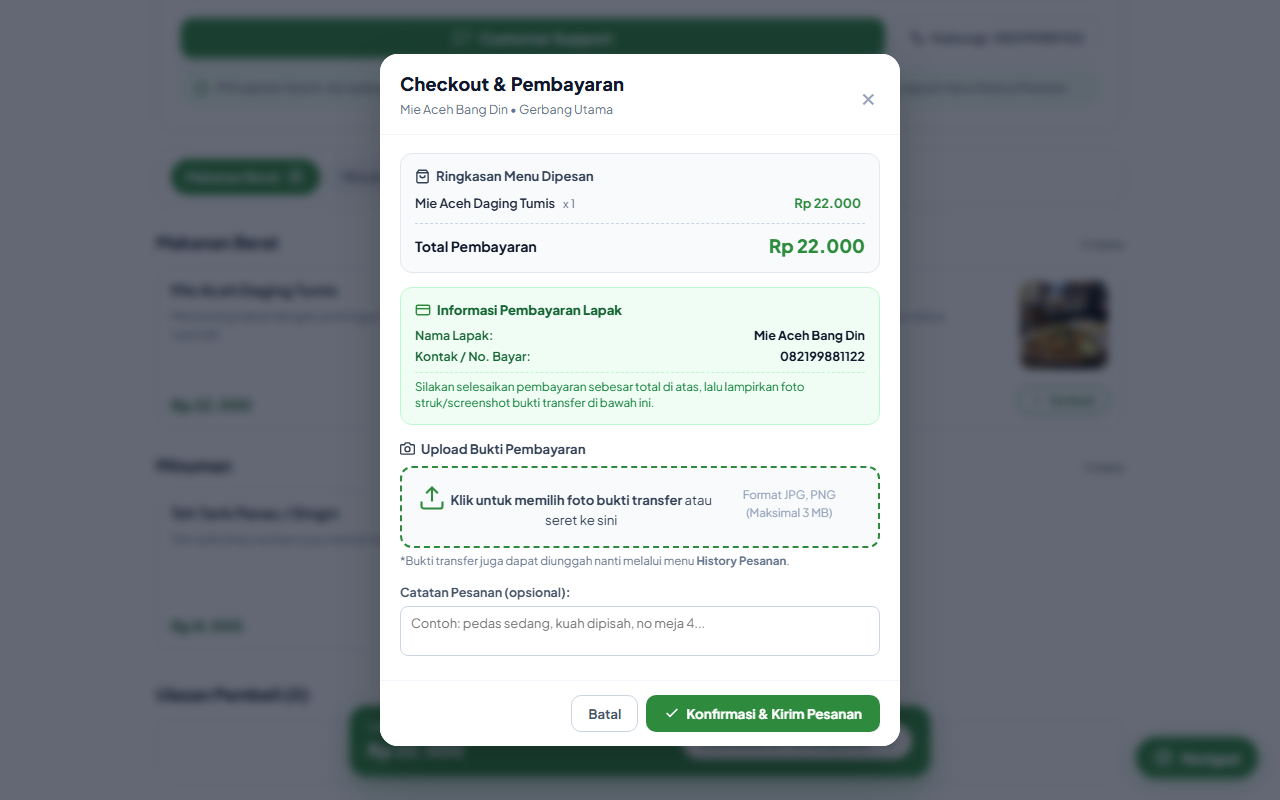
\includegraphics[width=\textwidth]{assets/screens/05_checkout_modal.png}
  \par\small (b) Modal \textit{Checkout} \& Unggah Bukti (F006/F007)
\end{minipage}
\caption{Antarmuka \textit{Frontend} Keranjang per Lapak dan Modal \textit{Checkout}}
\label{fig:fe-checkout}
\end{figure}

\subsection{Laci History Pesanan dan Unggah Ulang Bukti (\texttt{floating-chat.blade.php})}
Untuk pesanan yang belum melampirkan foto saat \textit{checkout} atau ditolak oleh Admin, pengguna mengunggah bukti melalui laci \textit{History Pesanan} (Gambar~\ref{fig:fe-history}):
\begin{enumerate}[leftmargin=1.5em, itemsep=2pt, topsep=2pt]
  \item \textbf{Pemuatan Riwayat (\texttt{loadOrderHistory}):} mengambil data dari \texttt{api.orders.history}, menampilkan daftar item, total harga, catatan penolakan Admin (\texttt{catatan\_admin}), serta pratinjau bukti yang sudah diunggah.
  \item \textbf{Visibilitas Tombol Unggah:} tombol ``Upload Bukti Bayar'' atau ``Perbarui Bukti'' (\texttt{bukaUploadBukti\allowbreak DariHistory}) hanya dirender bila \texttt{status\_pembayaran} bernilai \texttt{belum\_bayar} atau \texttt{ditolak}.
  \item \textbf{Validasi \& Pengiriman Bukti (\texttt{proofForm}):} memvalidasi keberadaan berkas serta batas ukuran 3~MB pada \texttt{proofFileInput}, lalu mengirim \texttt{FormData} ke rute \texttt{api.orders.upload\_bukti} dan memuat ulang isi laci tanpa keluar dari halaman aktif.
\end{enumerate}

\begin{figure}[htbp]
\centering
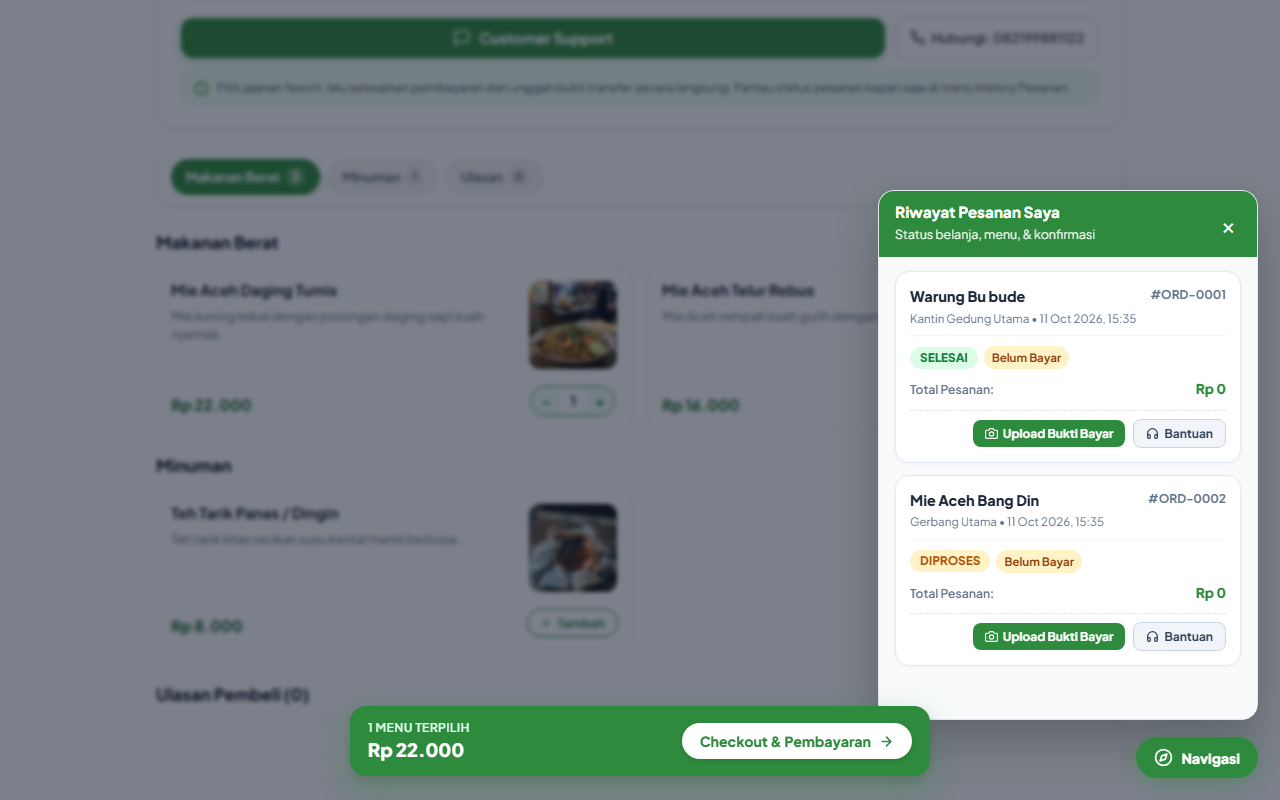
\includegraphics[width=0.52\textwidth]{assets/screens/06_history_drawer.png}
\caption{Antarmuka Laci \textit{History Pesanan} untuk Pemantauan \& Unggah Bukti (F007)}
\label{fig:fe-history}
\end{figure}

\section{Tahapan Implementasi Backend Logic (\texttt{ChatController.php})}

Seluruh logika bisnis dan keamanan data F006 serta F007 dipusatkan pada kelas kontroler \texttt{ChatController}:

\begin{enumerate}[leftmargin=1.5em, itemsep=2pt, topsep=2pt]
  \item \textbf{Validasi Sesi \& Masukan (\texttt{checkoutOrder}):} memeriksa pengguna melalui \texttt{getPengunjungId()} (\texttt{HTTP 401} jika belum masuk), mendecode JSON string \texttt{items} dari \texttt{FormData}, lalu memvalidasi \texttt{id\_umkm}, \texttt{items}, \texttt{catatan} (maks.\ 500 karakter), dan \texttt{bukti\_foto} (\texttt{image|mimes:jpeg,png,jpg|max:3072}).
  \item \textbf{Verifikasi Ketersediaan \& Anti-Manipulasi Harga:} memastikan lapak aktif melalui \texttt{Umkm::tampil()\allowbreak ->find(\$idUmkm)}. Pada setiap item, server membaca \texttt{Produk} milik lapak terkait; bila \texttt{!\$produk->tersedia}, server menolak transaksi dengan \texttt{HTTP 422}. Harga satuan diambil langsung dari kolom \texttt{harga} basis data (\texttt{\$qty * (int) round(\$produk->harga)}) sehingga nominal yang dimanipulasi di sisi klien diabaikan.
  \item \textbf{Penyimpanan Pesanan \& Bukti Awal:} jika \texttt{bukti\_foto} dilampirkan, berkas disimpan ke disk \texttt{public/bukti\_pembayaran/}, status bayar disetel menjadi \texttt{menunggu\_verifikasi}, dan \texttt{waktu\_\allowbreak pembayaran} dicatat. Jika tidak dilampirkan, status disetel \texttt{belum\_bayar}. Data dicatat ke \texttt{t\_pesanan} dengan \texttt{status = 'diproses'}.
  \item \textbf{Unggah Susulan \& Proteksi Status Lunas (\texttt{uploadBuktiPembayaran}):} memvalidasi \texttt{id\_pesanan} milik \texttt{\$idPengunjung} (\texttt{HTTP 404} jika bukan miliknya). Jika \texttt{\$pesanan->status\_pembayaran === 'lunas'}, server menolak permintaan dengan \texttt{HTTP 400}. Jika valid, foto baru disimpan, \texttt{status\_pembayaran} diubah menjadi \texttt{menunggu\_verifikasi}, dan \texttt{catatan\_admin} direset menjadi \texttt{null}.
\end{enumerate}

\needspace{7.5cm}
\begin{lstlisting}[language=PHP,caption={Inti Logika Validasi Harga Server \& Tolak Menu Habis di \texttt{ChatController::checkoutOrder}}]
foreach ($items as $item) {
    $produk = Produk::where('id_produk', (int) $item['id_produk'])
        ->where('id_umkm', $idUmkm)->first();
    if (!$produk || !$produk->tersedia) {
        return response()->json([
            'status' => 'error',
            'message' => 'Menu sedang habis / tidak tersedia pada lapak ini.',
        ], 422);
    }
    $qty = (int) $item['qty'];
    $harga = (int) round($produk->harga); // Harga asli server
    $subtotal = $qty * $harga;
    $totalHarga += $subtotal;
    $itemsDetail[] = [
        'id_produk' => $produk->id_produk, 'nama_produk' => $produk->nama_produk,
        'harga' => $harga, 'qty' => $qty, 'subtotal' => $subtotal,
    ];
}
\end{lstlisting}

\section{Hasil Verifikasi Pengujian Otomatis}

Pengujian fungsional otomatis dijalankan menggunakan PHPUnit (\texttt{php artisan test}) dengan \texttt{DatabaseTransactions} dan \texttt{Storage::fake('public')} pada berkas uji \texttt{F006F007CheckoutTest.php}. Seluruh skenario verifikasi dinyatakan lulus:

\renewcommand{\arraystretch}{1.20}
\begin{tabularx}{\textwidth}{|L{5.2cm}|Y|C{1.8cm}|}
\hline
\rowcolor{TableHeadBg}
\textbf{Skenario Pengujian} & \textbf{Asersi Terverifikasi} & \textbf{Status} \\
\hline
\texttt{guest\_cannot\_checkout} & Tamu tanpa sesi masuk ditolak \texttt{HTTP 401} (\texttt{unauthenticated}). & \textcolor{JajanGreen}{\textbf{PASS}} \\
\hline
\texttt{f006\_checkout\_computes\_\allowbreak server\_total\_saves\_note\_\allowbreak and\_blocks\_unavailable\_menu} & Harga manipulatif klien (\texttt{Rp1}) diabaikan; \texttt{total\_harga} dihitung dari \texttt{t\_produk}; \texttt{catatan\_pembeli} tersimpan; menu habis (\texttt{tersedia=false}) ditolak \texttt{HTTP 422}. & \textcolor{JajanGreen}{\textbf{PASS}} \\
\hline
\texttt{f007\_upload\_payment\_proof\_\allowbreak at\_checkout\_and\_history\_\allowbreak and\_block\_when\_lunas} & Upload saat \textit{checkout} \& via \textit{History Pesanan} mengubah status ke \texttt{menunggu\_verifikasi}; unggah ulang saat status \texttt{lunas} ditolak \texttt{HTTP 400}. & \textcolor{JajanGreen}{\textbf{PASS}} \\
\hline
\end{tabularx}

\vspace{0.25cm}
\noindent Total hasil eksekusi \texttt{php artisan test}: \textbf{5 passed (15 assertions)} dalam waktu \textbf{1,91 detik} (termasuk \texttt{ExampleTest} unit \& feature).

\end{document}
